\chapter{Grundlagen der Signalverarbeitung}

Ein \emph{Signal} ist eine Funktion eines Parameters mit numerischen Wertebereich. Die Abbildung zwischen Defintions- und Wertebereich kann, aber muss nicht durch eine Formel definiert sein. So fällt $f(x) = \sin( x )$ genauso unter die Definition eines Signals wie eine Folge numerischer Werte, die durch die Aufnahme eines Messgerätes enstanden sind. Weiterhin kommt dem Wertebereich eine gewissen Bedeutung zu, wie \emph{Zeit} oder \emph{Ort}. Ein typisches Beispiel für ein Signal ist die Spannung, die abhängig von der Zeit von einem Mikrofon erzeugt wird.  Da in dieser Arbeit nur Signale von Bedeutung sind, deren Wertebereich sich auf die Zeit bezieht, konzetrieren sich alle folgenden Bereich auf diesen Bereich- Im Zusammenhang mit Signalen wird der Definitionsbereich auch als \emph{unabhängiger Parameter} und der Wertebereich auch als \emph{abhängiger Parameter} bezeichnet. \cite[S. 11-12]{dspGuide} \cite[S. 22-23]{dspMichigan}

 Bei einem zeit-kontinuierlichen Signal $x( t )$ ist der Wertebereich kontinuierlich, wie in Formel  \ref{eq:time-cont-signal} definiert. Bei einem zeit-diskreten Signal $x[n]$ ist der Wertebreich diskret, wie in Formel \ref{eq:time-disc-signal} definiert. So beschreibt beispielsweise $x[17] = s$ den Wert zur Zeit $n = 17$. \glqq Zeit\grqq{} hat in diesem Kontext keine Einheit. Ein Wert wird auch als \emph{Sample} oder \emph{Amplitude} bezeichnet. $x[17] $ meint somit das 17. Sample des Signals. Abbildung \ref{img:aSignal} zeigt Beispiele für ein zeit-kontinuierliches und ein zeit-diskretes Signal. \cite[S. 22 - 23]{dspMichigan}

\begin{equation}
x(t) = s \; , t \in \mathbb{R}
\label{eq:time-cont-signal}
\end{equation}

\begin{equation}
x[n] = s \; , n \in \mathbb{Z} 
\label{eq:time-disc-signal}
\end{equation}

\begin{figure}
	\centering
	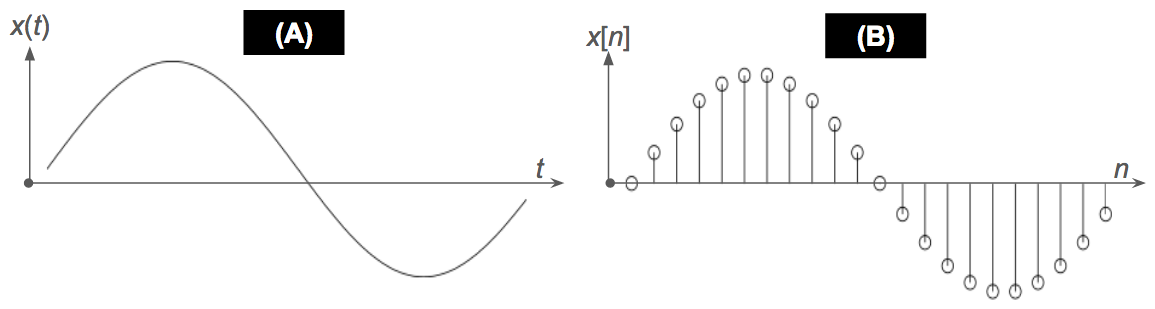
\includegraphics[width=0.6\textwidth]{bilder/aSignal02.png}
	\caption{Ein zeit-kontinuierliches Signal (A) und ein zeit-diskretes Signal (B)}
	\label{img:aSignal}
\end{figure}

Zeit-diskrete Signale werden häufig dadurch gewonnen, dass ein zeit-kontinuierliches Signal in regelmäßigen Intervallen abgetastet wird. Dieser Prozess wird als \emph{Sampling} bezeichnet und durch Formel \ref{eq:sampling} definiert. Der Parameter $T_s$ wird als \emph{Sampling-Interval} bezeichnet. Das Reziproke $\frac{1}{T_s} = f_s$ heißt \emph{Sampling-Rate} und wird in der Einheit $\frac{1}{\text{s}} = \text{Hz}$. Eine Sampling-Rate von $f_s = \SI{44100}{\hertz}$ bedeutete beispielsweise, dass ein Signal 44100 mal pro Sekunde abgetastet wurde.\cite[S. 24]{dspMichigan}

\begin{equation}
x[n] = s(n \cdot T_s) \; , -\infty < n < \infty
\label{eq:sampling}
\end{equation}
	
Da in dieser Arbeit nur zeit-diskrete Signale von Interesse sind, werden ab diesem Punkt die Definitonen für zeit-kontinuierliche Signale ausgelassen. Der \emph{Support} ist das kleinst mögliche Zeitintervall, der alle Samples enthält, die nicht den Wert 0 haben, wie Formel \ref{eq:support} definiert. Die \emph{Dauer} eines Signales ist die Länge des Supportes nach Formel . Das Signal $x[n] = \cos(n) \: ,0\leq n \leq 3$ hat beispielsweise den Support $[0,3] = \{0,1,2,3\} $ und die Dauer $4$. \cite[S. 24]{dspMichigan}

\begin{equation}
\begin{split}
\text{Sup}(x) = [sup_s, sup_e] \quad , sup_s, sup_e \in \mathbb{Z} \\,  x[sup_s] \neq 0 \:  \wedge \:  x[sup_e] \neq 0 \: \wedge \: \forall n \
\not\in [sup_s, sup_e] : x[n] = 0
\end{split}
\end{equation}

\begin{equation}
\text{Duration}(x) = sup_e - sup_s + 1
\label{eq:duration}
\end{equation}

Ein Signal gilt als \emph{periodisch}, wenn Formel \ref{eq:periodicity} erfüllt ist. Der Parameter $N$ wird als \text{Periode} von $x$ bezeichnet. Wenn ein Signal mit $N$ periodisch ist, dann ist es auch mit $2N, 3N, \ldots $ periodisch. Die Grundfrequenz $N_0$ ist das kleinste N, für das Formel \label{eq:periodicity} erfüllt ist. \cite[S. 24]{dspMichigan}

\begin{equation}
\exists N : \forall n \in Sup : x[n+N] = x[n] \rightarrow \text{Periodisch}(x,N) = true
\label{eq:periodicity}
\end{equation}
	

\section{Statistische Merkmale von Signalen}
\section{Faltung}
\section{Transformationen}
\subsection{Fourier-Transformation}
\subsection{Laplace-Transformation}
\subsection{Z-Transformation}
\section{Filter}
\section{akustische Modellierung der menschlichen Stimme}
\section{Feststellung von Periodizität in Signalen}
\subsection{Zero-Crossing-Rate}
\subsection{Methoden des Frequenzbereiches}
\subsection{Autokorrelation}
\subsection{Cepstrum}